
\chapter{基本理论}\label{chapter2}
\vbox{}\vbox{}

本章主要介绍与本文有关的一些理论背景知识。在第一节我们先从光场的量子化开始介绍了光与原子的相互作用等知识,然后第二节我们介绍了自旋压缩态的概念、判据以及产生等知识,再后第三节我们也介绍了关于纠缠的一些理论,包括纠缠的概念、纠缠的分类以及应用,最后第四节我们也介绍了海森堡朗之万理论的知识。
%第一节先介绍一下光场量子化的理论知识。第二节介绍光场与物质相互作用的理论知识。第三节介绍与海森堡-朗之万理论相关的一些理论知识。第四节则简单了介绍了一下腔QED相关的理论知识。
%光与物质的相互作用是量子光学里最基本的问题之一,单模电磁场与二能级原子的相互作用是电磁场与原子相互作用最简单、最基本的相互作用形式。本节以单模光场与二能级原子的相互作用为例,第一小节介绍原子与场相互作用系统的哈密顿量,第二小节介绍单模光场与二能级原子相互作用的半经典理论,第三小节介绍单模光场与二能级原子相互作用的全量子理论。
\vspace{1cm}
\section{光与原子相互作用}
\vspace{1cm}
\subsection{光场的量子化}
为了量化自由空间中的电磁场,可以方便地从基于麦克斯韦方程的场的经典描述开始。下面的这些方程分别将电场强度$\bm{E}$和磁场强度$\bm{H}$与电位移矢量和磁感应矢量$\bm{D}$和$\bm{B}$相关联,在真空中麦克斯韦方程组\cite{pennarun2007tripartite}的表现形式为(在mks单位下)
\begin{align}
\nabla  \times \bm{ H} &=    \frac{{\partial \bm{ D}}}{{\partial t}},\label{eq1}\\
\nabla  \times \bm{ E} &=  - \frac{{\partial \bm{ B}}}{{\partial t}},\label{eq2}\\
\nabla  \cdot  \bm{ B} &= 0,\label{eq3}\\
\nabla  \cdot  \bm{ D} &= 0,\label{eq4}
\end{align}
它们之间满足
\begin{align}
\bm{ B} &= {\mu _0}\bm{H},\label{eq5}\\
\bm{ D }&= {\epsilon_0}\bm{ E},\label{eq6}
\end{align}
其中$\epsilon_0$和$\mu_0$分别是自由空间的介电常数和磁导率,与光速$c$之间的关系为${\mu _0}{\epsilon_0} = {c^{ - 2}}$。下面,对方程(\ref{eq2})两边取旋度,使用方程(\ref{eq1})和(\ref{eq4}-\ref{eq6})可得电场强度$\bm{E}(\bm{r},t)$满足的波动方程
\begin{align}
	{\bm{\nabla} ^2}\bm{E} - \frac{1}{{{c^2}}}\frac{{{\partial ^2}\bm{E}}}{{\partial {t^2}}} = 0,\label{eq7}
\end{align}
其中,使用了关系式$\bm{\nabla } \times \left( {\bm{\nabla}  \times \bm{E}} \right) = \bm{\nabla } \cdot \left( {\bm{\nabla } \cdot \bm{E}} \right) - {\bm{\nabla} ^2}E$。

我们首先考虑电场具有适合于长度为L的空腔谐振器的空间依赖性。我们将电场在$x$方向上线性极化并在空腔的一般模式下展开
\begin{align}
{E_x}\left( {z,t} \right) = \sum\limits_j {{A_j}{q_j}\sin \left( {{k_j}z} \right)} ,\label{eq8}
\end{align}
其中
\begin{align}
{k_j} &= \frac{{j\pi }}{L},j = 1,2,3,...,\label{eq9}\\
{A_j} &= {\left( {\frac{{2v_j^2{m_j}\pi }}{{V{_0}}}} \right)^{1/2}},\label{eq10}
\end{align}
其中${v_j} = j\pi c/L$是腔的本征频率,$V$是谐振腔的体积,${m_j}$是一个与质量有关的常数,${q_j}$是位置坐标。同样,可将磁场模式化展开
\begin{align}
{H_y}\left( {z,t} \right) = \sum\limits_j {{A_j}\left( {\frac{{{{\dot q}_j}{_0}}}{{{k_j}}}} \right)\cos \left( {{k_j}z} \right)} ,\label{eq11}
\end{align}
电磁场的经典哈密顿量为
\begin{align}
H = \frac{1}{2}{\smallint _V}d\tau \left( {{_0}E_x^2 + {\mu _0}H_y^2} \right),\label{eq12}
\end{align}
其中积分为对整个腔体积分。将式(\ref{eq8})和式(\ref{eq11})代入式(\ref{eq12})中,我们得到
\begin{align}
H = &\frac{1}{2}\sum\limits_j {\left( {{m_j}v_j^2q_j^2 + {m_j}\dot q_j^2} \right)} \nonumber\\
= &\frac{1}{2}\sum\limits_j {\left( {{m_j}v_j^2q_j^2 + \frac{{p_j^2}}{{{m_j}}}} \right)} ,\label{eq13}
\end{align}
式中${p_j} = {m_j}{\dot q_j}$是第$j$个腔模的正则动量。

为了将光场量子化,我们引入了两个算符$p_j$和$q_j$,它们满足对易关系
\begin{align}
\left[ {{q_j},{p_{j'}}} \right] = i\hbar {\delta _{jj'}},\label{eq14}\\
\left[ {{q_j},{q_{j'}}} \right] = \left[ {{p_j},{p_{j'}}} \right] = 0,\label{eq15}
\end{align}
为了方便起见,我们再引入两个新算符$a_j$和$a_j^\dagger$
\begin{align}
{a_j}{e^{ - i{v_j}t}}& = \frac{1}{{\sqrt {2{m_j}\hbar {v_j}} }}\left( {{m_j}{v_j}{q_j} + i{p_j}} \right),\label{eq16}\\
a_j^\dag {e^{i{v_j}t}}& = \frac{1}{{\sqrt {2{m_j}\hbar {v_j}} }}\left( {{m_j}{v_j}{q_j} - i{p_j}} \right),\label{eq17}
\end{align}
接下来,$a_j$和$a_j^\dagger$的表达式代入式(\ref{eq13}),则哈密顿量变为
\begin{align}
H = \hbar {\rm{ }}\sum\limits_j {{v_j}\left( {a_j^\dag {a_j} + \frac{1}{2}} \right)} ,\label{eq18}
\end{align}
$a_j$表示系统的湮灭算符,$a_j^\dagger$表示系统的产生算符,当算符$a_j$作用在量子系统的态上时,系统湮灭一个光子,当算符$a_j^\dagger$作用在量子系统的态上时,系统产生一个光子。由算符$p_j$和$q_j$所满足的对易关系易式我们可以轻易地推导出$a_j$和$a_j^\dagger$满足的对易关系为
\begin{align}
\left[ {{a_j},a_{j'}^\dag } \right]& = {\delta _{jj'}},\label{eq19}\\
\left[ {{a_j},{a_{j'}}} \right] &= \left[ {a_{j}^\dag ,a_{j'}^\dag } \right]{\rm{ = }}0,\label{eq20}
\end{align}
将$a_j$和$a_j^\dagger$代入方程(\ref{eq8})和方程(\ref{eq11})可以得到由$a_j$和$a_j^\dagger$描述的电磁场表达式为
\begin{align}
{E_x}\left( {z,t} \right) &= \sum\limits_j {{\varepsilon _j}\left( {{a_j}{e^{ - i{v_j}t}} + a_j^\dag {e^{i{v_j}t}}} \right)\sin \left( {{k_j}z} \right)} ,\label{eq21}\\
{H_y}\left( {z,t} \right) &=  - i{_0}c\sum\limits_j {{\varepsilon _j}\left( {{a_j}{e^{ - i{v_j}t}} - a_j^\dag {e^{i{v_j}t}}} \right)\cos \left( {{k_j}z} \right)} ,\label{eq22}
\end{align}
其中${\varepsilon _j} = \left( \hbar v_j /\epsilon_0 V\right)^{1/2}$。

以上讨论的电磁场是处于一维有限腔中的情况,如果将一维腔拓展成为三维腔,其结果将变为如下的形式
\begin{align}
\bm{ E}\left( {\bm{ r},t} \right)& = \sum\limits_{\bm{ k}} {{{\hat\epsilon }_{\bm{ k}}}{\epsilon_{\bm{ k}}}{a_{\bm{ k}}}{e^{ - i{v_{k}}t + i\bm{ k} \cdot\bm{r}}} + H.c.} ,\label{eq23}\\
\bm{ H}\left( {\bm{ z},t} \right)& = \frac{1}{{{\mu _0}}}\sum\limits_{\bm{ k}} {\frac{{\bm{ k} \times {{\hat \epsilon}_{\bm{ k}}}}}{{{v_k}}}{\varepsilon _{\bm{ k}}}{a_{\bm{ k}}}{e^{ - i{v_k}t + i\bm{ k} \cdot \bm{r}}} + H.c.} , \label{eq24}
\end{align}
其中$H.c.$表示厄米共轭,$\bm{ k}$为波矢,有$\bm{ k}{\rm{ = }}\frac{{2\pi }}{L}\left( {{{\bm{ e}}_x}{n_x} + {{\bm{ e}}_y}{n_y} + {{\bm{ e}}_z}{n_z}} \right)$,其中$n_x,n_y,n_z =  \pm 1, \pm 2, \pm 3,...$,${\hat \epsilon_{\bm{ k}}}$为单位极化矢量,由方程(\ref{eq4})可以得到$\bm{k} \cdot {\hat \epsilon_{\bm{ k}}} = 0$,所以对于每个$\bm{k}$有两个独立的极化方向。

\subsection{原子-场相互作用的哈密顿量}\label{subsection21}

一个电量为$e$,质量为$m$的电子受到电磁场的作用,可以用如下的哈密顿量描述
\begin{align}
H = \frac{1}{{2m}}{\left[ {\bm{P} - e\bm{A}(\bm{r},t)} \right]^2} + eU(\bm{r},t) + V(\bm{r}),\label{eq25}
\end{align}
式中$\bm{P}$是正则动量算符($\bm{P} =  - i\hbar \bm{\nabla} $),$\bm{A}(\bm{r},t)$和$U(\bm{r},t)$分别是电磁场的矢势和标势,$V(\bm{r})$是静电势,一般是指原子的束缚势。

描述自由电子运动的薛定谔方程为
\begin{align}
H\psi (\bm{r},t) = i\hbar \frac{{\partial \psi(\bm{r},t) }}{{\partial t}},\label{eq26}
\end{align}
将式(\ref{eq25})代入式(\ref{eq26})得到
\begin{align}
\left\{ { - \frac{{{\hbar ^2}}}{{2m}}{{\left[ {\bm{\nabla}  - i\frac{e}{\hbar }\bm{A}(\bm{r},t)} \right]}^2} + e(\bm{r},t) + V(\bm{r})} \right\}\psi(\bm{r},t)  = i\hbar \frac{{\partial \psi(\bm{r},t) }}{{\partial t}},\label{eq27}
\end{align}
在$t$时刻,在$\bm{r}$处找到电子的概率密度用波函数$\psi(\bm{r},t)$的模方表示
\begin{align}
P\left( {\bm{r},t} \right) = {\left| {\psi \left( {\bm{r},t} \right)} \right|^2},\label{eq28}
\end{align}
由上式可以知道,波函数相差一个相位因子不会影响其概率密度,但是当相位因子随时间和空间变化时
\begin{align}
\psi '\left( {\bm{r},t} \right) = \psi \left( {\bm{r},t} \right){e^{i\chi (\bm{r},t)}},\label{eq29}
\end{align}
此时却不满足薛定谭方程($\chi$为任意常数相位)。为了使其还能满足薛定谔方程,
%\begin{align}H\psi  = i\hbar \frac{{\partial \psi }}{{\partial t}},\label{eq30}\end{align}
我们需要修正$\bm{A}(\bm{r},t)$和$U(\bm{r},t)$
\begin{align}
\bm{A}(\bm{r},t) \to &\bm{A}(\bm{r},t) + \frac{\hbar }{e}\nabla \chi (\bm{r},t),\label{eq31}\\
U(\bm{r},t) \to &U(\bm{r},t) - \frac{\hbar }{t}\frac{{\partial \chi (\bm{r},t)}}{{\partial t}},\label{eq32}
\end{align}
$\bm{A}(\bm{r},t)$和$U(\bm{r},t)$分别被识别为电磁场的矢量和标势。

我们现在研究一个电子被电位$V(\bm{r})$束缚在原子核附近$\bm{r}_0$处的问题。通过使用偶极近似,可以将原子与辐射场之间的相互作用的最小耦合哈密顿量简化为简单形式。原子处在平面电磁波中,电磁波用矢势$\bm{A}(\bm{r}_0+\bm{r},t)$描述,在偶极近似($\bm{k} \cdot\bm{ r} \ll 1$)下\cite{cc1998roc},该矢量势可以用偶极子近似值$\bm{k}·\bm{r} \ll 1$表示
\begin{align}\label{eq33}
  \begin{split}
     \bm{A}({\bm{r}_0} + \bm{r},t)& = \bm{A}(t)\exp [i\bm{k}({\bm{r}_0} + \bm{r})]\\
                   &= \bm{A}(t)\exp (i\bm{k} \cdot {\bm{r}_0})(1 + i\bm{k} \cdot \bm{r} +  \cdots )\\
                   &= \bm{A}(t)\exp (i\bm{k} \cdot {\bm{r}_0}),
  \end{split}
\end{align}
在偶极近似下,这个问题的薛定谔方程将由方程(\ref{eq27})和$\bm{A}(\bm{r},t) \equiv \bm{A}(\bm{r}_0,t)$给出,即
\begin{align}
\left\{ { - \frac{{{\hbar ^2}}}{{2m}}{{\left[ {\nabla  - i\frac{e}{\hbar }\bm{A}(\bm{r}_0,t)} \right]}^2} + eU(\bm{r},t) + V(\bm{r})} \right\}\psi(\bm{r},t)  = i\hbar \frac{{\partial \psi(\bm{r},t) }}{{\partial t}},\label{eq34}
\end{align}
电磁场的矢势和标势在库伦规范\cite{griffiths2005introduction}下
\begin{align}
\bm{\nabla}  \cdot \bm{A} &= 0\label{eq35}\\
         U(\bm{r},t) &= 0,\label{eq36}
\end{align}
定义一个新的波函数$\phi(\bm{r},t)$ ,薛定谔方程(\ref{eq34})可以简化为
\begin{align}
\psi (\bm{r},t) = \exp [\frac{{ie}}{\hbar }A({\bm{r}_0},t) \cdot \bm{r}] \cdot \phi (\bm{r},t),\label{eq37}
\end{align}
由方程(\ref{eq31}-\ref{eq37})可以得到$\phi(\bm{r},t)$满足的薛定谔方程为
\begin{align}
[ - \frac{{{\hbar ^2}}}{{2m}} + V(\bm{r})]\phi (\bm{r},t) = i\hbar \frac{{\partial \phi (\bm{r},t)}}{{\partial t}},\label{eq38}
\end{align}
又由
\begin{align}
\bm{E} =  -\bm{ \nabla} \cdot\bm{ U }- \frac{{\partial \bm{A}}}{{\partial t}},\label{eq39}
\end{align}
可以将方程(\ref{eq38})改写为
\begin{align}
({H_0} + {H_I})\phi (\bm{r},t) = i\hbar \frac{{\partial \phi (\bm{r},t)}}{{\partial t}},\label{eq40}
\end{align}
其中
\begin{align}
{H_0} &= \frac{{{p^2}}}{{2m}} + V(\bm{r}),\label{eq41}\\
{H_I} &=  - e\bm{r} \cdot E({\bm{r}_0},t),\label{eq42}
\end{align}
分别是电子的自由哈密顿量和系统的相互作用哈密顿量。

\subsection{单模光场与二能级原子相互作用的半经典描述}\label{subsection22}

\begin{figure}[htbp]
	\centering
	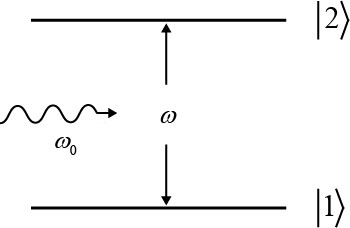
\includegraphics[scale=0.5]{Img/Fig_1.jpg}
	\bicaption{经典场与二能级原子相互作用示意图}{Schematic diagram of interaction between classical field and two-level atom}	\label{figure}
\end{figure}

如图\ref{figure}中,我们用$\ket{1}$和$\ket{2}$表示二能级原子的基态和激发态,能量本征值分别为$\hbar \omega_1$和$\hbar \omega_2$,经典场的频率为$\omega_0$。一个单模场与这个系统发生相互作用,描述系统的哈密顿量为
\begin{align}
H = {H_0} + {H_I} = \hbar {\omega _1}\left| 1 \right\rangle \left\langle 1 \right| + \hbar {\omega _2}\left| 2 \right\rangle \left\langle 2 \right| - er \cdot E(\bm
{r},t),\label{eq43}
\end{align}
其中
\begin{align}
{H_0} = \hbar {\omega _1}\left| 1 \right\rangle \left\langle 1 \right| + \hbar {\omega _2}\left| 2 \right\rangle \left\langle 2 \right|,\label{eq44}
\end{align}
为原子的自由哈密顿量。相互作用哈密顿量为
\begin{align}\label{eq45}
\begin{split}
{H_I} &=  - e\bm{r} \cdot E(t)\\
      &= - e\left( {\left| 1 \right\rangle \left\langle 1 \right| + \left| 2 \right\rangle \left\langle 2 \right|} \right) \cdot \bm{r} \cdot \left( {\left| 1 \right\rangle \left\langle 1 \right| + \left| 2 \right\rangle \left\langle 2 \right|} \right)E\left( t \right)\\
      &=  - e\left( {{u_{12}}{\sigma _{12}} + {u_{21}}{\sigma _{21}}} \right)E\left( t \right)
\end{split}
\end{align}
上面我们用到了关系式$\sum_i\sigma_{ii}=1$,$\sigma_{ij}=\ket{j}\bra{j}$是原子算符,$u_{12}=u_{21}^*=e\bra{1}r\ket{2}$是跃迁偶极矩阵元。假设电场沿着$r$方向极化,在偶极近似的条件下,电场可表示为
\begin{align}
E(t) = {E_0}\cos (vt) = \frac{1}{2}{E_0}({e^{i{\omega _0}}} + {e^{ - i{\omega _0}t}}),\label{eq46}
\end{align}
为了方便表述,我们定义场的拉比频率
\begin{align}
\Omega  = \frac{{{u_{21}}{E_0}}}{{2\hbar }},\label{eq47}
\end{align}
于是相互作用的哈密顿量可以写为
\begin{align}
{H_I} =  - \hbar \left( {{\Omega ^*}{\sigma _{12}} + \Omega {\sigma _{21}}} \right)({e^{i{\omega _0}}} + {e^{ - i{\omega _0}t}}),\label{eq48}
\end{align}
在相互作用绘景下,通过对相互作用哈密顿量做幺正变换,我们得到
\begin{align}\label{eq49}
\begin{split}
{V_I} =& {e^{i{H_0}t}}{H_I}{e^{ - i{H_0}t}}\\
      =&  - \hbar \Omega {\sigma _{21}}{e^{i\left( {\omega  - {\omega _0}} \right)t}} - \hbar {\Omega ^*}{\sigma _{12}}{e^{ - i\left( {\omega  - {\omega _0}} \right)t}}\\
&- \hbar \Omega {\sigma _{21}}{e^{i\left( {\omega  + {\omega _0}} \right)t}} - \hbar {\Omega ^*}{\sigma _{12}}{e^{ - i\left( {\omega  + {\omega _0}} \right)t}},
\end{split}
\end{align}
其中$\omega=\omega_2-\omega_1$。在上式中我们采用旋转波近似,略去两个快速振荡的项之后,系统的哈密顿量最终可以变为如下的形式
\begin{align}
{V_I} =  - \hbar \Omega {\sigma _{21}}{e^{i\left( {\omega  - {\omega _0}} \right)t}} - \hbar {\Omega ^*}{\sigma _{12}}{e^{ - i\left( {\omega  - {\omega _0}} \right)t}}.\label{eq50}
\end{align}

\subsection{单模光场与二能级原子相互作用的全量子描述}\label{paf}

\begin{figure}[htbp]
	\centering
	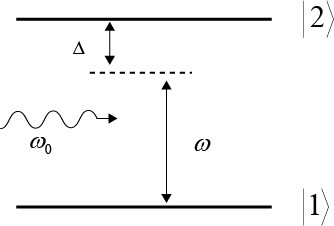
\includegraphics[scale=0.5]{Img/Fig_2.jpg}
	\bicaption{单模光场与二能级原子相互作用示意图}{Schematic diagram of interaction between single-model field and two-level atom}	\label{figure2}
\end{figure}

全量子描述就是将光场和原子都做了量子化处理。单模场与单个二能级原子的相互作用是量子光场与物质相互作用的最简单模型,称为拉比模型,取旋转波近似后的形式称为Jaynes-Cummings模型(简称J-C模型)。

如图\ref{figure2}所示,原子的自由哈密顿量为
\begin{align}
{H_A} = \hbar {\omega _1}\left| 1 \right\rangle \left\langle 1 \right| + \hbar {\omega _2}\left| 2 \right\rangle \left\langle 2 \right|,\label{eq51}
\end{align}
选取能量零点使得$\hbar {\omega _2}{\rm{ = }}\frac{1}{2}\hbar \omega$,$\hbar {\omega _1}{\rm{ = }} - \frac{1}{2}\hbar \omega$, $\omega  = {\omega _2} - {\omega _1}$,并引入泡利算符${\sigma _z} = \left| 2 \right\rangle \left\langle 2 \right| - \left| 1 \right\rangle \left\langle 1 \right|$,则有
\begin{align}
{H_A} = \frac{1}{2}\hbar {\omega _0}{\sigma _z},\label{eq52}
\end{align}

单模光场的自由哈密顿量为
\begin{align}
{H_F} = \hbar {\omega _0}{a^\dag }a,\label{eq53}
\end{align}
上式中略去了与光场自由哈密顿量无关紧要的常数项$\hbar \omega/2$。

相互作用的哈密顿量为
\begin{align}\label{eq54}
\begin{split}
{H_I} &= \sum\limits_{j,k} {\sum\limits_\lambda  {\hbar {g_{jk,\lambda }}} } \left| j \right\rangle \left\langle k \right|({a_\lambda } + a_\lambda ^\dag )\\
&= \sum\limits_{j,k} {\hbar {g_{jk}}\left| j \right\rangle \left\langle k \right|(a + {a^\dag })} \\
&= \left( {\hbar {g_{21}}\left| 2 \right\rangle \left\langle 1 \right| + \hbar {g_{12}}\left| 1 \right\rangle \left\langle 2 \right|} \right)(a + {a^\dag })\\
&= \hbar \lambda \left( {\left| 2 \right\rangle \left\langle 1 \right| + \left| 1 \right\rangle \left\langle 2 \right|} \right)(a + {a^\dag })\\
&= \hbar \lambda \left( {{\sigma ^{\rm{ + }}} + {\sigma ^ - }} \right)(a + {a^\dag }),
\end{split}
\end{align}
其中${\sigma ^ + }{\rm{ = }}\left| 2 \right\rangle \left\langle 1 \right|$,${\sigma ^ - } = \left| 1 \right\rangle \left\langle 2 \right|$,并假设$g_{21}=g_{12}=\lambda$。

于是可得,系统的总的哈密顿量为
\begin{align}\label{eq55}
\begin{split}
H &= {H_A} + {H_F} + {H_I}\\
&= \frac{1}{2}\hbar {\omega _0}{\sigma _z} + \hbar {\omega _0}{a^\dag }a + \hbar \lambda \left( {{\sigma ^ + } + {\sigma ^ - }} \right)(a + {a^\dag }),
\end{split}
\end{align}
上式中,相互作用哈密顿量中四项的物理意义分别为:$\sigma^+a$表示原子吸收一个光子从低能级跃迁到高能级;$\sigma^-a^\dagger$表示原子从高能级跃迁到低能级并放出一个光子;$\sigma^-a$表示原子从高能级跃迁到低能级的同时吸收一个光子;$\sigma^+a^\dagger$表示原子从低能级跃迁到高能级的同时放出一个光子。

在旋转波近似下,略去方程(\ref{eq55})中能量不守恒的项以后,系统的哈密顿量变为
\begin{align}
H = \frac{1}{2}\hbar {\omega _0}{\sigma _z} + \hbar {\omega _0}{a^\dag }a + \hbar \lambda \left( {{\sigma ^ + }a + {\sigma ^ - }{a^\dag }} \right),\label{eq56}
\end{align}
将上式变换到相互作用绘景,可得相互作用绘景中的相互作用哈密顿量为
\begin{align}
{H_I} = \hbar \lambda \left( {{\sigma ^ + }a{e^{i\Delta t}} + {a^\dag }{\sigma ^ - }{e^{ - i\Delta t}}} \right),\label{eq57}
\end{align}
其中$\omega-\omega_0$为原子和场的失谐量。

J-C模型虽然是在基于电偶极近似与旋转波近似的前提下推导出来的,但是由于J-C模型是可积的,即可以得到精确解析的结果,所以它的重要性不言而喻,而正因为如此,所以它也成为了在量子光学中研究问题的一个最基本的模型。
而它之所以重要并不仅在于其模型可精确求解的缘故,更在于它预测了一系列的实验结果,比如拉比震荡(Rabi oscillating)\cite{rabi1937space,cummings2013reminiscing},原子布居数的坍塌-复苏\cite{rempe1987observation,eberly1980periodic},真空中的自发辐射过程,光子反聚束\cite{haroche2013nobel,wineland2013nobel},纠缠\cite{rauschenbeutel2000step,phoenix1991establishment}以及亚迫松分布等。

















\vbox{}
\section{自旋压缩态}
\vbox{}
压缩态概念最早的出现是在光学中,由于压缩态很多非经典态所没有的特性,因此对压缩态的研究显得格外重要。由于压缩光在光学高精度测量中可以降低光子计数噪声、提高非破坏性%(quantum nondemolition, QND)
测量的灵敏度和光通信等方面有着重要的应用,所以被引入到自旋系统,称之为自旋压缩态。自旋压缩态与光的压缩态相比在存储和保真度方面更容易实现,而且在量子信息的研究方面扮演着很重要的角色,故而关于自旋压缩态的研究受到了广泛的关注。

本节内容主要介绍了一些关于自旋压缩态的一些概念,包括光场压缩态的相关知识、自旋压缩态的基本概念、定义和压缩参数等内容。

\subsection{光场的压缩态}\label{section31}

压缩态的概念最先存在于光学中,最初由David Stole提出,在上个世纪七八十年代开始压缩光由于在引力波测量、精密测量以及光通信等方面的重要应用而受到重视。

光场的湮灭算符$a$和产生算符$a^\dagger$可按实部与虚部展开:
\begin{align}
	a = {X_1} + i{X_2},{a^\dag } = {X_1} - i{X_2},\label{eq331}
\end{align} 
由于$a$和$a^\dagger$之间的对易关系满足
\begin{align}
	\left[ {a,{a^\dag }} \right] = 1,\label{eq332}
\end{align}
因此可以得到
\begin{align}
	\left[ {{X_1},{X_2}} \right] = i/2,\label{eq333}
\end{align}
引入$A,B$两个算符,根据海森堡不确定度关系我们可以得到
\begin{align}\label{eq334}
	V\left( A \right)V\left( B \right) \ge \frac{1}{4}{\left| {\left\langle {\left[ {A,B} \right]} \right\rangle } \right|^2},
\end{align}
于是有
\begin{align}\label{eq335}
	V\left( {{X_1}} \right)V\left( {{X_2}} \right) \ge \frac{1}{{16}},
\end{align}
其中,$V\left( {{X_i}} \right)\left( {i = 1,2} \right)$为正交分量$X_i$的方差。

引入标准偏差$\Delta A \equiv \sqrt {V\left( A \right)} $,则式(\ref{eq334})和式(\ref{eq335})又可表示为
\begin{align}
	&( \Delta A)(\Delta B) \ge \frac{|\braket{[A,B]}|^2}2,\label{eq336}\\
	&( \Delta X_1)( \Delta X_2) \ge 1/4,\label{eq337}
\end{align}
在公式(\ref{eq337})中取等号的态我们将其称之为最小的不确定度态,即相干自旋态%(coherent spin state, CSS)
。当$\Delta X_1^2\left( {\Delta X_2^2} \right) < 1/4$时,如果有$\Delta X_2^2\left( {\Delta X_1^2} \right) >1/4$,而此时海森堡不确定度关系依旧成立,我们可以看到其中有一个不确定度已经小于相干态的量子涨落所能达到的最小值(1/4),产生了压缩现象,因此我们就称此时光场处于压缩态。这就是光场压缩态的定义。

\subsection{自旋压缩的定义}

在研究自旋压缩的过程中,自旋压缩的定义并不是唯一的,它取决于具体研究的系统,目前被广泛接受的定义是由Kitagawa和Ueda类似于光的压缩态提出的定义\cite{PRA1993Kitagawa},以及Wineland等人\cite{PRA1994Wineland}在研究Ramsey实验时提出的定义。除了这两个被广泛研究的定义之外,还有一些其他的自旋压缩定义\cite{sorensen2001many,toth2009spin,wang2010sudden}被提出,这些定义是为了某些考虑而引入的。

受到光场的压缩态启发,类比于光场的压缩,K. W\'odkliewicz和Eberly\cite{wodkiewicz1987k}这么定义了自旋压缩态:
将自旋算符$\mathbf{S}$在三维的直角坐标轴上正交分解为$S_x$,$S_y$和$S_z$,它们之间满足对易关系
\begin{align}
	\left[ {{S_x},{S_y}} \right] = i{S_z}\left( {\hbar  = 1} \right),\label{eq338}
\end{align}
此时,根据海森堡不确定度关系我们将得到
\begin{align}
	{\left( {\Delta {S_x}} \right)^2}{\left( {\Delta {S_y}} \right)^2} \ge \frac{{{{\left| {\left\langle {{S_z}} \right\rangle } \right|}^2}}}{4},\label{eq339}
\end{align}
当$(\Delta S_x)^2=(\Delta S_y)^2=\braket{ S_z}/2$时,系统就处于相干态。如果$(\Delta S_i)^2<\braket{S_z}/2$$(i=x,y)$,则系统此时处于自旋压缩态。

这个看似合理的定义实际上是不具完备性的,因为它仅仅只是通了过坐标系的旋转就将相干自旋态变成了自旋压缩态,这显然是不正确的。在证明这个定义不正确之前,我们先来证明一下相干态的实质是所有的自旋都沿着同一个方向极化的态。我们这里假设所有的方向都指向$z$轴的正方向,则系统所处的态可以表示为$\ket{S,S}$,我们在这个态下计算各个原子自旋分量的平均值及平方的平均值我们将得到如下的结果:
\begin{align}\label{eq3310}
	\begin{split}
		\braket{S_x}    &= \braket{S_y}  = 0,	\braket{S_z}  = S,\\
		\braket{S_x^2}  &= \bra{S,S}(\frac{S_++S_-}2)^2\ket{S,S} \\
		            	&= \bra{S,S}S_+S_-\ket{S,S}/4\\
		            	&= S/2,\\
		\braket{S_y^2}  &= \bra{S,S}(\frac{S_+-S_-}{2i})^2\ket{S,S} \\
		            	&= \bra{S,S}S_+S_-\ket{S,S}/4\\
			            &= S/2,\\
		(\Delta S_x)^2  &= (\Delta S_y)^2 = \braket{S_z}/2,
	\end{split}
\end{align}
现在我们将证明这个定义为什么不正确。假设一个系统最初处于相干态,平均自旋指向$z$轴正方向(如图\ref{figure3}所示),即$\braket{S}=\braket{S_z}$,则有$(\Delta S_x)^2  = (\Delta S_y)^2 = \braket{S_z}/2$,如果将$y$-$z$平面绕着$x$轴旋转一个角度$\theta$,$y$,$z$到达新的位置$y'$,$z'$。
\begin{figure}[h!]
	\centering
	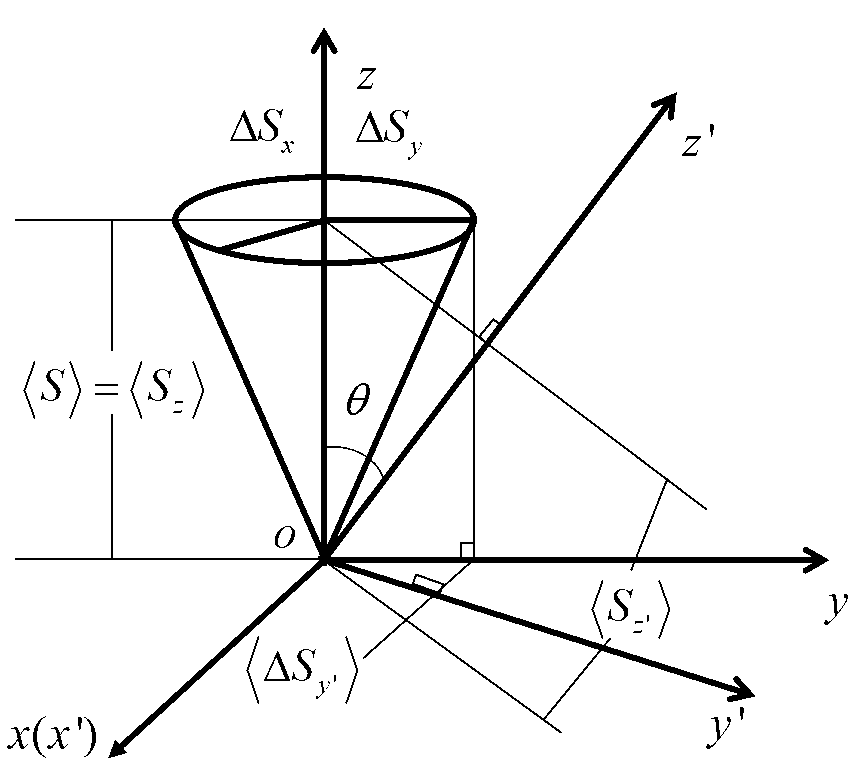
\includegraphics[scale=0.45]{Img/Fig_3.png}\\
	\vspace{0.5cm}
	\bicaption{角动量及其变化量在不同坐标系中的投影}{Projection of angular momentum and its variation in different coordinate systems}	\label{figure3}
\end{figure}

在新的坐标系中,因为:
\begin{align}\label{eq3312}
	\begin{split}
		\Delta S_{x'} & = \Delta {S_x}\\
		\braket{S_{z'}} & = \braket{S_{z'}}  \cos \theta \\
		\Delta {S_{y'}} & = \Delta {S_y}\cos \theta ,
	\end{split}
\end{align}
所以有
\begin{align}\label{eq3313}
	\begin{split}
		\Delta S_{x'}^2 &= \frac{\braket{S_z}}{2} \ge \frac{\braket{S_{z'}}}{2}\\
		\Delta S_{y'}^2 &= \Delta S_y^2~{\cos ^2}\theta  \le \frac{\braket{S_z}}{2}\cos \theta  = \frac{\braket{S_{z'}}}{2},
	\end{split}
\end{align}
如果$\theta\ne 0$,$\Delta S_{x'}^2 > \braket{S_{z'}}/2$,$\Delta S_{y'}^2 < \braket{S_{z'}}/2$。根据上述自旋压缩的定义,在$x'y'z'$坐标系中系统现在处于压缩态。

上述的证明表明在这样的定义下,仅仅只是通过旋转了坐标系,系统便由原来的相干态转化成压缩态,这显然是不正确的,因为通过旋转坐标并没有对系统进行任何操作,系统没有发生任何变化。而且,旋转坐标只是通过哈密顿量的线性作用,而光压缩的产生需要非线性哈密顿量的作用才可以产生,因此这个定义显然是不合理的。

在这个基础上Kitagawa和Ueda提出了更加普遍的定义,他们认为,考察的对象应该是垂直于总自旋方向的自旋分量,如果这个分量的最小不确定量的平方小于相干态所能达到的最小值,则系统便是处于自旋压缩态。为了计算方便,在选择坐标时一要尽量使系统的平均总自旋处于直角坐标轴上。

\subsection{自旋压缩的数学表示}

考虑由$N$个1/2自旋的原子组成的系综,这个自旋1/2原子系综的角动量算符由下式给出
\begin{align}
	{J_\alpha } = \frac{1}{2}\sum\limits_{l = 1}^N {{\sigma _{l\alpha }}} ,\alpha  = x,y,z,\label{eq3314}
\end{align}
其中$\sigma_{l\alpha}$是第$l$个原子的泡利矩阵。在讨论自旋压缩态之前,先介绍一下相干自旋态(Coherent spin state, CSS)。

CSS可以写成单个自旋态的直积形式
\begin{align}
	\left| {\theta ,\phi } \right\rangle  = \mathop  \otimes \limits_{l = 1}^N \left[ {\cos \frac{\theta }{2}{{\left| 0 \right\rangle }_l} + {e^{i\phi }}\sin \frac{\theta }{2}{{\left| 1 \right\rangle }_l}} \right],\label{eq3315}
\end{align}
其中$\ket{0}_l$和$\ket{1}_l$表示算符$\sigma_{lz}$的本征值分别为1和-1的本征态,在上式的定义中,所有的自旋都指向同一个方向。利用下式
\begin{align}
	\exp \left[ {i\left( {\xi {\sigma _ + } + \eta {\sigma _ - }} \right)} \right] = \cos \sqrt {\xi \eta }  + i\frac{{\sin \sqrt {\xi \eta } }}{{\sqrt {\xi \eta } }}\left( {\xi {\sigma _ + } + \eta {\sigma _ - }} \right),\label{eq3316}
\end{align}
可以将CSS写成如下的形式
\begin{align}
	\left| {\theta ,\phi } \right\rangle  = \mathop  \otimes \limits_{l = 1}^N {R_l}\left( {\theta ,\phi } \right){\left| 0 \right\rangle _l} = \mathop  \otimes \limits_{l = 1}^N \exp \left( {\varsigma {\sigma _ + } - {\varsigma ^*}{\sigma _ - }} \right){\left| 0 \right\rangle _l},\label{eq3317}
\end{align}
其中
\begin{align}
	\varsigma  =  - \frac{\theta }{2}\exp \left( {i\phi } \right),\label{eq3318}
\end{align}
更进一步地可以将CSS表示为
\begin{align}
	\ket {\theta ,\phi }  = {R_l}(\theta ,\phi )\ket {j,j}= \exp ( {\varsigma {J_ + } - {\varsigma ^*}{J_ - }} )\ket {j,j}  ,\label{eq3319}
\end{align}
其中
\begin{align}
	\left| {j,j} \right\rangle  \equiv \mathop  \otimes \limits_{l = 1}^N {\left| 0 \right\rangle _l},\label{eq3320}
\end{align}
$\ket{j,j}$表示算符$J_z$本征值为$j=N/2$的本征态,这就意味着所有的自旋分量都在$z$轴方向上。其中
\begin{align}
	{J_ \pm } = {J_x} \pm i{J_y},\label{eq3321}
\end{align}
为跃迁算符,$R\left( {\theta ,\phi } \right)$为旋转算符,由下面的式子给出
\begin{align}
	R\left( {\theta ,\phi } \right) = \exp \left( { - i\theta {J_{\vec n}}} \right) = \exp \left[ { - i\theta \left( {{J_x}\sin \phi  - {J_y}\cos \phi } \right)} \right],\label{eq3322}
\end{align}
其中$\vec n = \left( { - \sin \phi ,\cos \phi ,0} \right)$。

角动量算符的对易关系
\begin{align}
	\left[ {{J_\alpha},{J_\beta}} \right] = i{\varepsilon _{\alpha\beta\gamma}}{J_\gamma},\label{eq3323}
\end{align}
其中$\alpha,\beta,\gamma$表示任意三个正交方向的分量。$\varepsilon _{\alpha\beta\gamma}$是Levi-Civita符号。不确定关系是
\begin{align}
(\Delta J_\alpha)^2(\Delta J_\beta)^2\ge |\braket{ J_\gamma}|^2/4,\label{eq3324}
\end{align}
当上式左边的两个涨落中有一个满足
\begin{align}\label{eq3325}
	\begin{split}
	(\Delta J_\beta)^2\le |\braket{ J_\gamma}|/2,
	\end{split}
\end{align}
我们就说这个系统是被压缩的。也就是说,由于原子之间非经典关联的缘故\cite{PRA1993Kitagawa},在不违法海森堡不确定度关系的前提下,两个正交分量的不确定度被重新分配,其中一个角动量分量的不确定度将小于标准量子极限。这种自旋角动量在某个方向的涨落减小的态称为自旋压缩态。

对于一个原子系统,如果各个原子之间未能产生量子关联,则其各个原子的自旋分量的方向应该沿空间各方向平均自由分布,在垂直于平均自旋的平面内的任意相互垂直的两个方向上都分布着相同的总自旋,没有压缩性质的存在,如图(a)所示的自旋角动量。如果自旋角动量的涨落在某一方向上部分地减小,则表明在各个自旋单体之间建立起某种关联,正是这种量子关联效应导致了自旋压缩,如图(b)所示,而这种压缩同时也导致了其垂直方向上涨落的增加,压缩的增加与海森堡不确定关系仍旧成立,这是自旋压缩的基本原理。我们也可以把处于自旋压缩态的自旋矢量设想成一个椭圆形圆锥,如图\ref{figure4}所示。
\begin{figure}[htbp]
	\centering
	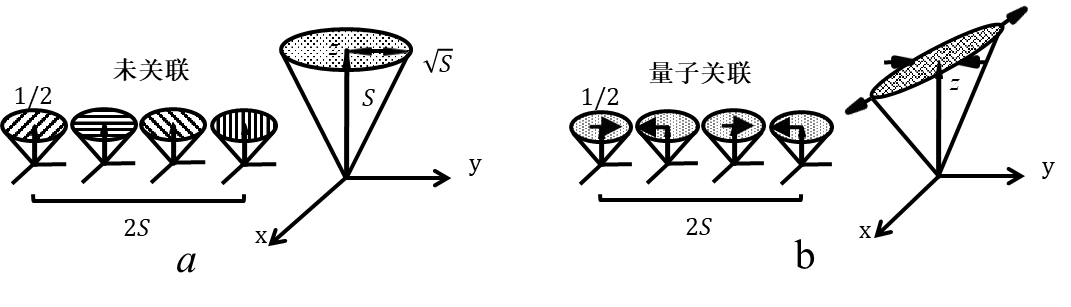
\includegraphics[scale=0.78]{Img/Fig_4.png}
	\bicaption{
		2S个独立的自旋1/2原子的S个自旋态的示意图。
		(a) 2S个未关联的1/2自旋构成的相干自旋态。
		(b) 2S个关联的1/2自旋构成的自旋压缩态。}
	{Schematic illustrations of S-spin states in terms of 2S individual 1/2 spins. 
		(a) Coherent spin state constructed from 2S uncorrelated 1/2.
		(b) Squeezed spin state constructed from 2S correlated 1/2.
	}	
	\label{figure4}
\end{figure}


\subsection{自旋压缩参数}

对于一个特定的系统而言,其自旋压缩一般是利用自旋压缩系数来进行判定的。关于自旋压缩系数的定义,相关文献\cite{MA201189}中论及的有好几种,但究竟哪一种是最好的到目前都还没有定论。比较典型的是Kitagawa和Ueda给出的定义以及Wineland等人给出的定义。下面我们分别来看一下这两种定义。

Kitagawa和Ueda给出的定义:
\begin{align}
	\xi _K^2 = \frac{{2\min {{\left( {\Delta {J_{{{\vec n}_ \bot }}}} \right)}^2}}}{j} = \frac{{4\min {{\left( {\Delta {J_{{{\vec n}_ \bot }}}} \right)}^2}}}{N},\label{eq3326}
\end{align}

Wineland等人给出的定义:
\begin{align}
	\xi _W^2 = \frac{{N{{\left( {\Delta {J_{{{\vec n}_ \bot }}}} \right)}^2}}}{{{{\left| {\left\langle {{J_{{{\vec n}_ \bot }}}} \right\rangle } \right|}^2}}},\label{eq3327}
\end{align}
在上式中,下标${\vec n_ \bot }$指的是与平均自旋方向$\vec n=\braket{J}/\sqrt{\braket{J}\braket{J}}$垂直的方向。对于相干自旋态,我们有$(\Delta {J_{{\vec n}_ \bot} })^2=j/2$,如果$J_{{\vec n}_ \bot} $小于$j/2$,则此时处于自旋压缩态。 ${J_{{{\vec n}_ \bot }}}=J \cdot {\vec n_ \bot }$可以利用方差${\left( {\Delta J} \right)^2}$的最小值来计算自旋压缩系数。如果上述表达式$\xi _K^2 \le 1\left( {\xi _W^2 \le 1} \right)$,则系统是自旋压缩的。$\xi _K^2 \le 1\left( {\xi _W^2 \le 1} \right)$的值越小,自旋压缩发生的程度越大。

我们先介绍Kitagawa和Ueda的定义,在式(\ref{eq3326})中$\min {\left( {\Delta {J_{{{\vec n}_ \bot }}}} \right)^2}$指垂直于平均自旋方向投影与垂直平面上的最小自旋不确定度。若给定了平均自旋角动量的方向
\begin{align}
	{\vec n_0} = \left( {\sin \theta \cos \phi ,\sin \theta \sin \phi ,\cos \theta } \right),\label{eq3328}
\end{align}
其中极化角和方位角分别为
\begin{align}\label{eq3329}
	\left\{ \begin{array}{ll}
		\theta&=\arccos (\braket{J_z}/|J|)\\
		\phi &= 2\pi + (\braket{J_y}/|\braket{J_y}|)\arccos (\braket{J_x}/|J\sin \theta|),
	\end{array} \right.
\end{align}
则垂直${\vec n_0}$的平面内的两个相互垂直的矢量为
\begin{align}\label{eq3330}
	\left\{ \begin{array}{ll}
		{\vec n_1} &= (-\sin\varphi, \cos\phi,0)\\
		{\vec n_2} &= (\cos\theta\cos\varphi, \cos\theta\sin\varphi, -\sin\varphi),
	\end{array} \right.
\end{align}
即满足${\vec n_0} \cdot {\vec n_1} = {\vec n_0} \cdot {\vec n_2} = {\vec n_1} \cdot {\vec n_2} = 0$,因此,在垂直于平均自旋角动量方向的平面内的任意自旋角动量方向总可以表示成
\begin{align}
	{\vec n_ \bot } = {\vec n_1}\cos \phi  + {\vec n_2}\sin \phi ,\label{eq3331}
\end{align}
于是,系统总的角动量在某矢量的投影可以表示为
\begin{align}
	{J_{{{\vec n}_ \bot }}} = J \cdot {\vec n_ \bot } = J \cdot {\vec n_1}\cos \phi  + J \cdot {\vec n_2}\sin \phi  = {J_{{n_1}}}\cos \phi  + {J_{{n_2}}}\sin \phi ,\label{eq3332}
\end{align}
将式(\ref{eq3326})带入$\Delta J_{{{\vec n}_ \bot }}^2$后,通过计算可得
\begin{align}\label{eq3333}
	\begin{split}
		\xi _K^2 &= \frac{2}{N}\min \left[ \braket{J_{n_1}^2 + J_{n_2}^2}+ \cos (2\theta)\braket{J_{n_1}^2 - J_{n_2}^2}\right] + \sin ( 2\theta )
		\braket{\left[ J_{n_1},J_{n_2} \right]_+ }^2\\
		&= \frac{2}{N}\left[\braket{J_{n_1}^2 + J_{n_2}^2}- \sqrt {\braket{J_{n_1}^2 - J_{n_2}^2} + \braket{\left[ J_{n_1},J_{n_2} \right]_+ }^2} \right],
	\end{split}
\end{align}



现在我们讨论Wineland等人提出的自旋压缩参数。在Ramsey光谱学的研究中。压缩参数ξR2是在Ramsey光谱中确定共振频率时一般状态和CSS之间的波动的比率。这里的CSS充当噪声参考状态。与ξS2相比,ξS2是玻色子压缩的类比,参数ξR2基本上与角动量状态对旋转的灵敏度的改善相关,因此对于实验是有吸引力的。




Wineland等人提出的定义是在研究Ramsey光谱学的时候提出来的,压缩参数$\xi_W$是在Ramsey光谱中确定共振频率时一般状态和CSS之间的涨落的比率。在实验中如果初态刚开始处于CSS,则相位不确定度为${\left( {\Delta \phi } \right)_{CSS}} = {1 / {\sqrt N }}$,把它称为标准量子极限。如果相位不确定度满足${\left( {\Delta \phi } \right)_{CSS}} <{1 / {\sqrt N }}$,我们就称其处于自旋压缩态。他们的定义为
\begin{align}
	\xi _W^2 = \frac{{{{\left( {\Delta \phi } \right)}^2}}}{{\left( {\Delta \phi } \right)_{CSS}^2}} = \frac{{N\left( {\Delta {J_{{n_ \bot }}}} \right)}}{{{{\left| {\left\langle J \right\rangle } \right|}^2}}},\label{eq3334}
\end{align}
一般情况下,$|\braket{J}| \le  N/2$,因此	
\begin{align}
	\xi _W^2 = \frac{{N\left( {\Delta {J_{{n_ \bot }}}} \right)}}{{{{\left| {\left\langle J \right\rangle } \right|}^2}}} \ge \frac{{N\left( {\Delta {J_{{n_ \bot }}}} \right)}}{N} = \xi _K^2,\label{eq3335}
\end{align}
我们可以看出来Kitagawa和Ueda的自旋压缩参数是从海森堡不确定关系出发的,考虑的是垂直于自旋方向的涨落和$J/2$的关系。而Wineland等人的定义则是从测量和参数估计出发,利用自旋压缩参数来看能突破标准量子极限的程度的。具体选用哪一种参数和具体研究的体系和问题有关系,这是目前使用最多的两种定义,除此之外还有一些其它的定义,祥见参考文献\cite{MA201189}。
\subsection{自旋压缩的产生}	

目前产生自旋压缩态的方法已经有很多种,但是大致可以归纳以下两类:

(1) 在原子系综中通过光与原子的相互作用产生自旋压缩态。非常自然的一个想法就是将光的压缩态转移到自旋系统,许多方案中也提到通过电磁感应透明来转移压缩。当考虑光原子相互作用时,光与原子之间的失谐是非常重要的。在大失谐的情况下,可以得到系统有效的哈密顿量,包括色散相互作用项和非线性相互作用项,并且可以调整这两个项的大小。  
  (a)光与原子之间的色散相互作用导致光的偏振的法拉第旋转。然后通过对输出光进行量子非破坏性(quantum nondemolition, QND)测量,可以将原子系综在测量结果的条件下压缩,该方法已经在实验中实现。  
  (b)描述原子间相互作用的非线性项是单轴扭曲哈密顿量,可用于产生自旋压缩。

(2) 在玻色-爱因斯坦凝聚(Bose–Einstein condensations, BEC)中通过原子之间的碰撞来产生自旋压缩态。
在过去十年中,在BEC中产生自旋压缩状态引起了相当大的兴趣。双组分BEC中的非线性原子-原子碰撞可以用单轴扭曲哈密顿量来描述,它通常用于产生自旋压缩态。此外,双轴扭转哈密顿量可以通过拉曼过程实现,也可以通过双阱势中的双组分冷凝物来实现。自旋压缩也可以通过自旋交换相互作用或自由动力学演化在自旋-1 BEC中产生。

自旋压缩产生的关键是在粒子之间产生相互关联,这种关联可以通过粒子之间的非线性相互作用来实现。在文献\cite{PRA1993Kitagawa}中,Kitagawa和Ueda不仅重新定义了自旋压缩态,与此同时还提出了两种用于产生自旋压缩非线性哈密顿量的模型:单轴扭曲模型(One-axis twisting Hamiltonian)和双轴扭曲模型的哈密顿量(two-axis twisting Hamiltonian)。接下来我们简单介绍一下这两种模型。

\subsubsection{单轴扭曲模型}

在基础自旋之间建立量子关联,需要非线性的相互作用。现在考虑一个由哈密顿量$H=\hbar F(S_z)$生成的幺正算符为$U(t)=exp[-itF(S_z)]$,通过这个幺正算符我们可以写出它的升降算符为${S_ \pm } \equiv {S_x} \pm i{S_y}$,其演化方式可以表述为如下的形式
\begin{align}
	{S_ + }\left( t \right) = {U^\dag }{S_ + }\left( 0 \right)U = {S_ + }\left( 0 \right)\exp \left[ {itf\left( {{S_z}} \right)} \right],\label{eq3336}
\end{align}
和${S_-}\left( t \right) = {\left[ {{S_ + }\left( t \right)} \right]^\dag }$,其中
\begin{align}
	f\left( {{S_z}} \right) = F\left( {{S_z}{\rm{ + }}1} \right) - F\left( {{S_z}} \right),\label{eq3337}
\end{align}
对于最低次幂的非线性相互作用$F(S_z)=\chi S_z^2$将导致$f(S_z) = 2\chi (S_z+1/2)$,即与$S_z$成比例的旋转,将量子涨落进行扭转。
扭转之后的角动量算符的$x$分量和$y$分量分别为${S_x}(t)= \frac12(S_+e^{i\mu(S_z+1/2)}+e^{-i\mu(S_z+1/2)}S_z)$和${S_y}(t)= \frac{1}{2i}(S_+e^{i\mu(S_z+1/2)}-e^{-i\mu(S_z+1/2)}S_z)$,其中$\mu  \equiv 2\chi t$。不确定度在$y-z$平面的正交分量上发生了重新分布,如图\ref{figure5}所示。
\begin{figure}[h!]
	\centering
	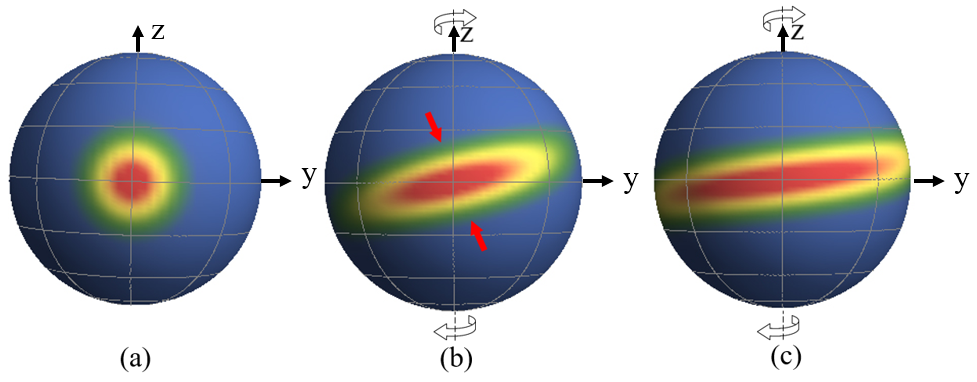
\includegraphics[scale=0.42]{Img/oat2.png}
	\bicaption{当S=20时,准概率分布(quasi-probability distribution, QPD)表示出的单轴扭曲模型所引起的态演化。图中的密度通过$Q(\theta,\phi)$最大值$Q_{max}$进行了归一化。(a)显示初始相干自旋态$\ket{\theta=\pi/2,\phi=0}(Q_{max}=1)$。(b)和(c)显示由$U=exp[-i\mu S_z^2/2]$产生的单轴扭曲模型的态; (b)最优压缩出现在$\mu=0.199(Q_{max}=0.445)$; (c)显示在$\mu=0.399(Q_{max}=0.241)$的过度扭曲。(c)中的QPD与测地线有所偏移。}
	{State evolutions by one-axis twisting in terms of the quasiprobability distribution (QPD) on the sphere for S = 20. The densities of the figures are normalized by the maximum value $Q_{max}$ of $Q(\theta,\psi)$. (a) shows the initial coherent spin state $\ket{\theta=\pi/2,\phi=0}(Q_{max}=1)$. (b) and (c) show one-axis twisted states generated by the unitary transformation $U=exp[-i\mu S_z^2/2]$; (b) optimally squeezed at $\mu=0.199(Q_{max}=0.445)$ and (c) excessively twisted at $\mu=0.399(Q_{max}=0.241)$. Although not clear from the figure, the QPD of (c) deviates from a geodesic (swirliness).}
	\label{figure5}
\end{figure}
\subsubsection{双轴扭曲模型}

虽然OAT模型可以有效地产生自旋压缩,但其最佳压缩角度却与系统的尺寸和演化时间有着密切的关系。如果在垂直于平均自旋方向的平面中围绕两个正交轴顺时针和逆时针同时进行扭转,则可以完美的解决这个问题。如图\ref{figure6}所示,若初始态CSS$\ket{0,\phi}$沿$\theta=\pi/2$,$\phi=\pm \pi/4$两个轴进行反向扭转,双轴反向扭曲的哈密顿量可以写成
\begin{align}
	H  = \chi(S_{\pi/2,\pi/4}^2-S_{\pi/2,-\pi/4}^2)
	= \frac{\chi}{2i}(S_+^2-S_-^2),\label{eq3338}
\end{align}
在参考文献\cite{helmerson2001creating,zhang2003entanglement,wesenberg2002mixed}提出了几种如何产生这个哈密顿量的方法。

当S较小时,双轴扭曲的自旋压缩态可以达到的最小方差小于1/2,随着S增大,最小方差趋近于1/2。当被压缩的方差达到1/2时,增强方差可以达到$S^2/2$。当$S^2/2$超过最优值时,QPD分成两个部分。双轴反向扭曲可以最大化地消除噪音。
\begin{figure}[h!]
	\centering
	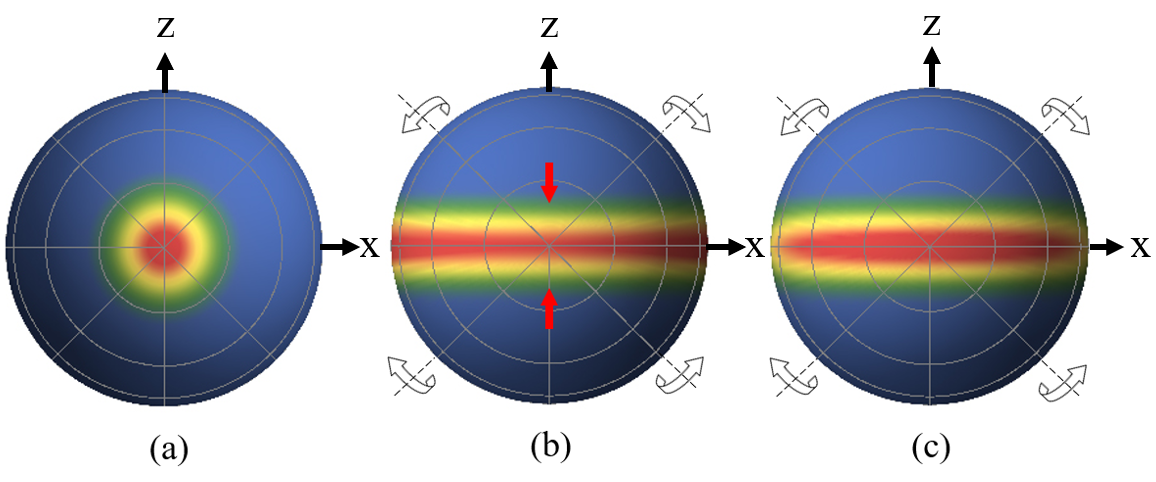
\includegraphics[scale=0.35]{Img/tat2.png}
	\bicaption{当S=20时,准概率分布(quasi-probability distribution, QPD)表示出的双轴反扭曲模型所引起的态演化。图中的密度通过$Q(\theta,\phi)$最大值$Q_{max}$进行了归一化。(a)显示初始相干自旋态$\ket{\theta=\pi/2,\phi=0}(Q_{max}=1)$。(b)和(c)显示由$U=exp[-i\mu(S_{\pi/2,\pi/4}^2-S_{\pi/2,-\pi/4}^2)/4]$产生的双轴反扭曲模型的态; (b)最优压缩出现在$\mu=0.203(Q_{max}=0.252)$; (c)显示在$\mu=0.248(Q_{max}=0.187)$的过度扭曲,QPD分裂为两部分。}
	{State evolutions by two-axis countertwisting in terms of the quasiprobability distribution (QPD) on the sphere for S=20. 
		The densities of the figures are normalized by the maximum value $Q(\theta,\phi)$ of $Q(\theta,\phi)$. 
		(a) shows the initial coherent spin state $\ket{\theta=\pi/2,\phi=0}(Q_{max}=1)$. 
		(b) and (c) are two-axis countertwisted states generated by the unitary transformation $U=exp[-i\mu(S_{\pi/2,\pi/4}^2-S_{\pi/2,-\pi/4}^2)/4]$; 
		(b) optimally squeezed at $\mu=0.203(Q_{max}=0.252)$ and (c) excessively twisted at $\mu=0.248(Q_{max}=0.187)$, where the QPD splits into two parts.}
	\label{figure6}
\end{figure}

双轴扭曲与单轴扭曲相比有以下的优点:在整个演化过程中,最佳压缩角度始终不变;压缩度比单轴扭曲模型高。单轴扭曲模型的压缩参数的最小值为$\xi_R^2\propto1/N^{2/3}$,而双轴扭曲可以达到海森堡极限$1/N$。


\vbox{}
\section{量子纠缠态}
\vbox{}
量子纠缠是一种量子力学现象,其中两个或更多粒子的量子态必须相互参照描述,即使各个物体可以在空间上分开。
它是量子信息中一个基本概念,也是几乎所有量子信息处理中不可缺少的理论支撑,其在不同学科之间起到了一个桥梁的作用,利用它我们可以很好的研究一些由大量粒子组成的系统的的统计性质。在这一节中,我们主要介绍了量子纠缠的基本概念、度量方式、应用、以及常见的两粒子系统之间的量子纠缠态。

\subsection{量子纠缠的概念}
纠缠态的概念首先是由薛定谔于1935年发表的薛定谔的猫态一文\cite{article1935}中提出的。这篇文章里讲述了一个假想实验,在一个密封的箱子里有一只猫,箱子里有一个装满毒气的瓶子,而装毒气的瓶子是否破碎完全由一个放射装置控制。假设这个放射装置里的放射元素发生衰变的概率是50$\%$,也就是说如果里面的放射性元素发生衰变的话就会触动机关,毒药瓶就会破碎放出毒气,则猫被毒死。否则,则猫是活着的。薛定谔用如下的表达式来描述这个活猫和死猫的复合系统:
\begin{align}
\ket{\Psi}=\alpha\ket{live\  cat}\ket{\uparrow}+\beta\ket{dead\  cat}\ket{\downarrow},|\alpha|^2+|\beta|^2=1,
\end{align}
其中$|\alpha|^2$表示猫活着的概率,$|\beta|^2$表示猫死了的概率。从上面的表达式我们可以看出来,猫以不同的概率同时处于这两种状态,即猫同时处于活着和死了的叠加态。而只有我们打开这个箱子去观测它我们才能知道猫到底是死了还是活着。这么一来,猫的生死就无法依赖于观测之前的“客观事实”,而是依赖于我们的观测,这是哥本哈根学派给出的解释。由于量子世界与我们所生活的宏观世界的生活经验差异之大,所以一时间人们很难接受。而人们对于这种量子描述的质疑主要来自于量子纠缠表现出来的非局域性,于是在这种质疑下人们提出了量子纠缠的概念。
\subsection{几种常见纠缠态}
由于不同数目的粒子都有可能纠缠在一起,所以按照纠缠粒子数的多少可以将纠缠态分为以下几类:在两粒子纠缠的系统中,我们将这种纠缠态称之为Bell态\cite{bell1964einstein}(由于Bell等人提出了著名的Bell不等式的缘故)。在三粒子系统中则有两种纠缠模型,分别称之为GHZ态\cite{greenberger2000similarities}和W态\cite{dur2000three}。而对于多粒子的系统,则分别有对应的多粒子GHZ态,多粒子W态,Cluster态,Dicke态等其他的一些纠缠态。下面简单介绍一下。
\subsubsection{Bell态}
Bell态是爱尔兰的物理学Bell提出来用于描述两个qubit系统的最大纠缠态,其具体的表达式为
\begin{align}\label{eq2241}
\begin{split}
\ket{\psi^{\pm}}&=\frac{1}{\sqrt{2}}(\ket{0}_A\ket{1}_B\pm\ket{1}_A\ket{0}_B)\\
\ket{\phi^{\pm}}&=\frac{1}{\sqrt{2}}(\ket{0}_A\ket{0}_B\pm\ket{1}_A\ket{1}_B)
\end{split}
\end{align}
上面的这四个态统称为一组Bell基,它是四维Hilbert空间的正交归一完备的基矢。如果用这组Bell作为测量基矢对系统进行测量操作,这个过程叫做Bell基测量。我们接下来证明一下Bell态具有非定域关联性,先假设A和B构成了一个处于Bell态$\ket{\psi^\pm}$的系统,我们先对A进行量子测量,于是我们可能得到两种不同的测量结果:粒子A处于1态或0态,如果是A则B必定是0,反之B为1。也就是说这两个粒子之间有某种关联,即当我们对一个粒子进行测量的时候,另外一个粒子的测量结果我们也会得到。
\subsubsection{GHZ纠缠态}
GHZ态是一种三粒子纠缠系统,由三名科学家一起提出来的\cite{greenberger2000similarities},它的表达式为
\begin{align}\label{eq2242}
\ket{GHZ}=\frac{1}{\sqrt{2}}(\ket{0}_A\ket{0}_B\ket{0}_C\pm\ket{1}_A\ket{1}_B\ket{1}_C),
\end{align}
从公式(\ref{eq2242})我们可以看出来GHZ态也具有非局域关联性,即当测量其中一个粒子处于$\ket{1}$($\ket{0}$)态时,其它的两个也注定处于$\ket{1}$($\ket{0}$)态。
\subsubsection{W纠缠态}
W纠缠态是另外一种三粒子纠缠态,它的表达式为
\begin{align}\label{eq2243}
\ket{W}=\frac{1}{\sqrt{3}}(\ket{0}_A\ket{1}_B\ket{1}_C+\ket{1}_A\ket{0}_B\ket{1}_C+\ket{1}_A\ket{1}_B\ket{1}_C),
\end{align}
从上式我们可以看出,不同于GHZ态,当其中一个粒子处于$\ket{1}$态时,另外两个粒子将塌缩到两粒子纠缠态$\ket{1}\ket{0}+\ket{0}\ket{1}$。由于此性质,因此W态已经被广泛的运用到量子信息处理方案中\cite{lee2006quantum,xi2007controlled,hao2009scheme}。

\subsection{量子纠缠的度量}
类似于压缩态用压缩度来度量其压缩程度一样,我们也用纠缠度来度量量子纠缠的程度。纠缠度量描述的方法也各不一样,这里介绍几种比较常见的度量方法。
\subsubsection{约化熵纠缠}
假如系统是两体纯态,那么约化熵纠缠的定义\cite{phoenix1990periodicity,phoenix1991establishment}为
\begin{align}\label{eq2244}
E=S_N(\rho_A)=S_N(\rho_B),
\end{align}
其中$S(\rho_A)=-Tr(\rho_A\log\rho_A)$和$S(\rho_B)=-Tr(\rho_B\log\rho_B)$分别表示系统A,B的约化密度矩阵的化密度矩阵的冯·诺依曼嫡,其中对数函数的底2,$\rho_A=Tr_B(\ket{\Psi}_{AB}\bra{\Psi})$,$\rho_B=Tr_A(\ket{\Psi}_{AB}\bra{\Psi})$。如果我们已经知道系统A得约化密度矩阵$\rho_A$的本征值$\lambda_i$,则$S_N(\rho_A)$就要写为如下的形式:
\begin{align}\label{eq2245}
S_N(\rho_A)=-\sum_i\lambda_i\log\lambda_i,
\end{align}

如果在两体纯态基础上,考虑两体混合态的约化嫡,则有如下定义:
\begin{align}\label{eq2246}
E_I=S(\rho_A)+S(\rho_B)-S(\rho_{AB}),
\end{align}
把$E_I$定义为相对信息嫡。
\subsubsection{形成纠缠}
在一个两体系统中,如果体系量子态可以用$\rho_{AB}=\sum_i p_i\ket{\Psi_i}_{AB}\bra{\Psi_i}$表示,那么纠缠的定义可以写为\cite{zhang2007thermal}:
\begin{align}\label{eq2247}
E_F(\rho_{AB})=\mathop {\min }\limits_{{{\left\{ {{p_i},{{\left| {{\Psi _i}} \right\rangle }_{AB}}} \right\}}_i}} \sum\limits_i {{p_i}{E_p}({{\left| {{\Psi _i}} \right\rangle }_{AB}})} ,
\end{align}
其中min的下标表示所有$\rho_{AB}$的集合。$E_p(\ket{\Psi_i}_{AB})$表示$\ket{\Psi_i}_{AB}$
的约化熵纠缠。

Wootters等人后面又提出了进一步反映量子态纠缠度的概念-并发度。如果一个两体系统的密度矩阵为$\rho_{AB}$,那么它们之间的纠缠可以表示成如下的形式:
\begin{align}\label{eq2248}
E_F(\rho_{AB})=H(\frac{1+\sqrt{1-C^2(\rho_{AB})}}2),
\end{align}
在上式中$H(p)=-p\log_2p-(1-p)\log_2(1-p)$,$C(\rho_{AB})$就是并发度,具体的表达式为$C(\rho_{AB})=max{0,\lambda_1-\lambda_2-\lambda_3-\lambda_4}$,其中$\lambda_i$(i=1,2,3,4,且有$\lambda_1\ge\lambda_2\ge\lambda_3\ge\lambda_4$)
表示$R=\rho_{AB}(\sigma_y^A\otimes\sigma_y^B)\rho_{AB}^*(\sigma_y^A\otimes\sigma_y^B)$的本征值平方根。

如果系统的密度矩阵表示为
\begin{equation}\label{eq2249}
\rho_{A B}=\left( \begin{array}{cccc}{\rho_{11}} & {0} & {0} & {\rho_{14}} \\ {0} & {\rho_{22}} & {\rho_{23}} & {0} \\ {0} & {\rho_{32}} & {\rho_{33}} & {0} \\ {\rho_{41}} & {0} & {0} & {\rho_{44}}\end{array}\right)
\end{equation}

那么体系的并发度就可以具体表示为
\begin{equation}\label{eq2250}
C\left(\rho_{A B}\right)=2 \max \left\{0,\left|\rho_{23}-\sqrt{\rho_{11} \rho_{44}}\right|,\left|\rho_{14}-\sqrt{\rho_{22} \rho_{33}}\right|\right\}
\end{equation}

\subsection{量子纠缠的应用}
量子纠缠是一种很重要的资源,其在量子隐形传态,量子秘钥分发等方面有着很重要的应用。

\subsubsection{量子隐形传态}
在1993年Bennett等人\cite{bennett1993teleporting}提出了量子隐形传态的协议,其对于任意未知量子态之间的传输是通过利用EPR纠缠的方法来实现的。该协议的主要思想是空间上相隔很远的两个通讯者之间分享一个纠缠态,通过利用这个纠缠态并借助经典通信渠道,便可以全部的分享一个量子态。

下面我们具体的介绍一下这个协议的工作原理:

假设通讯的双方为Alice和Bob,现在Alice想把1粒子的信息发送给Bob,未知的量子态表示为:
\begin{align}\label{eq2251}
\ket{\Psi}_1=\alpha\ket{0}_1+\beta\ket{1}_1,
\end{align}
其中$\alpha,\beta$为概率幅,满足归一化条件:$\alpha^2+\beta^2=1$。由于Alice和Bob之间共享一对EPR纠缠态,这对纠缠态的表示为
\begin{align}\label{eq2252}
\ket{\Psi}_{23}=\frac{1}{\sqrt{2}}(\ket{0}_2\ket{0}_3+\ket{1}_2\ket{1}_3),
\end{align}
则Alice和Bob所有粒子构成系统的总的状态可以表示为:
\begin{equation}
\begin{aligned} | \Psi \rangle_{123} &=| \Psi \rangle_{1} \otimes | \Psi \rangle_{23} \\ 
&=\frac{1}{\sqrt{2}}(\alpha\ket{0}_1+\beta \ket{1}_1 ) \otimes( \ket{0}_2\ket{0}_3+\ket{1}_2\ket{1}_3 ) \\
 &=\frac{\alpha}{\sqrt{2}}( \ket{0}_1\ket{0}_2\ket{0}_3+\ket{0}_1\ket{1}_2\ket{1}_3)+\frac{\beta}{\sqrt{2}}( \ket{1}_1\ket{0}_2\ket{0}_3+\ket{1}_1\ket{1}_2\ket{1}_3 ) \end{aligned}
\end{equation}

接下来我们将粒子1和2分解到4个Bell基上:
\begin{equation}
\begin{aligned} 
\ket{\Phi^{\pm}}_{12}&=\frac12(\ket{0}_1\ket{0}_2\pm\ket{1}_1\ket{1}_2)\\
\ket{\Phi^{\pm}}_{12}&=\frac12(\ket{0}_1\ket{1}_2\pm\ket{1}_1\ket{0}_2),
\end{aligned}
\end{equation}
则这个系统可以重新表示为
\begin{equation}
\begin{aligned} 
\ket{\Psi}_{123}=&[\ket{\Phi^{+}}_{12}(\alpha\ket{0}_3+\beta\ket{1}_3)+\ket{\Phi^{-}}_{12}(\alpha\ket{0}_3-\beta\ket{1}_3)\\
                     +&  \ket{\Psi^{+}}_{12}(\alpha\ket{1}_3+\beta\ket{0}_3)+\ket{\Psi^{-}}_{12}(\alpha\ket{1}_3-\beta\ket{0}_3)]/2,
\end{aligned}
\end{equation}
Alice对粒子1和2进行Bell态测量,然后把测量结果反馈给Bob,  Bob根据Alice反馈的结果,对所拥有的3号粒子进行幺正操作,便可以得到未知态$\ket{\Psi}_3$。

量子隐形传态有以下的几个特点:
(1)要完成量子隐形传态除了需要量子通道之外,还需要借助经典通道才能完成,因此,此过程不会超光速,也就不违背光速最大原理。
(2)在整个传态过程中,Alice需要对手中的粒子进行测量,测量以后这个粒子便不再处于原来的状态,因此整个过程也不违背量子不可克隆定理。
(3)由于量子纠缠态的非局域特性,整个过程不受空间的限制,所以通讯双方无需知道对方在哪里都可以进行。

总的来说,量子隐形传态传输的是量子信息,但其传输过程仍需要经典通道的协助,不过经典通道只是传达了测量结果。所以,未知量子态的传输并未加在任何的载体上,便可在一个地方突然消失,又在另一个地方突然出现。
\subsubsection{量子秘钥分发}
量子密钥分发(KQD)是一种安全的通信方法,它实现了基于量子力学成分的加密协议,它使通信双方产生只有他们自己知道共享随机秘钥,然后可以用于加密和解密消息。QKD的安全性依赖于自然的基本定律,这些定律不受增加计算能力,新攻击算法或量子计算机的影响,它可以抵御任意的强大窃听者。

1984年,Bennett和Brassard首次提出利用光子的偏振态来实现量子密钥分配的协议,又称为BB84协议\cite{bennett1984brassard}。在BB84协议中,首先选择有四个偏振方向的线性偏振单光子,四个偏振方向分别为水平方向、垂直方向45$^{\circ}$和135$^{\circ}$方向,这四个方向的光子态分别用$\ket{H}$、$\ket{V}$、$\ket{L}=1/\sqrt{2}(\ket{H}+\ket{V})$和$\ket{R}=1/\sqrt{2}(\ket{H}-\ket{V})$表示,这四个量子态之间都彼此正交,各自组成一对测量基,前两个态组成的基称为直测量基$\oplus$,后者称为斜测量基$\otimes$。

\begin{table}[htbp]
	\centering
		\bicaption{BB84协议中双方操作过程}{The operation process of both parties in the BB84 protocol}
	\begin{tabular}{|c|c|c|c|c|c|c|c|c|}
		\hline  % 在表格最上方绘制横线
		Alice's random bit              &0&1&1&0&1&0&0&1\\
		\hline  %在第一行和第二行之间绘制横线
		Alice's random sending basis    &$+$&$+$&$\times$&$+$&$\times$&$\times$&$\times$&$+$\\
		\hline  %在第一行和第二行之间绘制横线
		Photon polarization Alice sends &$\uparrow$&$\rightarrow$&$\searrow$&$\uparrow$&$\searrow$&$\nearrow$&$\nearrow$&$\rightarrow$\\
		\hline  %在第一行和第二行之间绘制横线
		Bob's random measuring basis    &$+$&$\times$&$\times$&$\times$&$+$&$\times$&$+$&$+$\\
		\hline  %在第一行和第二行之间绘制横线
		Photon polarization Bob measures&$\uparrow$&$\nearrow$&$\searrow$&$\nearrow$&$\rightarrow$&$\nearrow$&$\rightarrow$&$\rightarrow$\\
		\hline  %在第一行和第二行之间绘制横线
		PUBLIC DISCUSSION OF BASIS      &&&&&&&&\\
		\hline  %在第一行和第二行之间绘制横线
		Shared secret key               &0&&1&&&0&&1\\
		\hline  %在第一行和第二行之间绘制横线
	\end{tabular}
\end{table}
我们现在来看一下BB84协议的执行过程是怎么样的:首先Alice随机选择一种偏振光子用${\ket{H},\ket{V},\ket{L},\ket{R}}$,然后通过量子通道将其发送给Bobo。在发送之前,Alice和Bob约定好了给光子量子态$\ket{H}$、$\ket{R}$编码为0,光子量子态用$\ket{V}$、$\ket{L}$编码为1。随后Bob按照之前约定好的光量子态随机选择一种测量对自己接收到的量子态进行测量,并记录下测量结果。完了之后Bob通过公开信道将自己选择的测量基和测量结果告诉Alice。Alice通过将Bob的结果与自己的发送态和测量基进行比较,然后通过同样的通道告诉Bob哪些结果需要保留,哪些需要丢弃。

最后我们简单的分析一下量子密钥分发的安全性。假设在密钥传输的过程中存在着一个非法窃听者Eve,Eve首先通过技术手段窃取了Alice发送的量子态,然后随即选择了一组测量基对其进行测量。Eve有50\%的概率选对测量基和50\%的概率选错测量基。为了自己在窃取过程中不被发现,Eve冒充Alice将测量结果发送给Bob。结果,Bob最终将以正确率为$50\%\times 100\%+50\%\times 50\%=75\%$的概率保留正确的结果,即窃听者Eve引起的误码率为25\%。如果Alice向Bob发送N个量子态,那么误码率为0.25$^N$,当N很大时,误码率接近于0,因此,我们可以下结论:量子密钥分配具有很高的安全性。

%\subsection{量子纠缠的产生}
\vbox{}
\section{海森堡-朗之万理论}\label{section23}
\vbox{}
利用我们前面第\ref{paf}小节得到的哈密顿量,我们可以很容易的写出海森堡-朗之万方程\cite{scully1998quantum}。对于一个跃迁频率为$\omega$的原子系综和腔场耦合的系统,其总的哈密顿量可以表示为如下的形式
\begin{align}
H = \frac{1}{2}\hbar {\omega _0}\sum\nolimits_j {\sigma _j^z}  + \hbar {\omega _0}{a^\dag }a + \hbar \lambda \sum\nolimits_j {\Theta \left( {t - {t_j}} \right)} \left( {\sigma _j^ + a + \sigma _j^ - {a^\dag }} \right),\label{eq58}
\end{align}
其中$\Theta \left( {t - {t_j}} \right)$一般称做阶跃函数。

在上面的哈密顿量中,$\sigma_j^+$和$\sigma_j^-$分别表示产生算符和湮灭算符。$\sigma_j^-$是第$j$个原子的布居差。根据海森堡方程我们可以计算得出如下的原子与场的演化方程
\begin{align}\label{eq59}
\begin{split}
\dot a &=  - \frac{\gamma }{2}a - i\lambda \sum\nolimits_j {\Theta \left( {t - {t_j}} \right)} \sigma _j^ +  + {F_a}\left( t \right),\\
\dot \sigma _j^ + & =  - \frac{\gamma }{2}\sigma _j^ +  + i\lambda \Theta \left( {t - {t_j}} \right)\left[ {\sigma _j^a - \sigma _j^b} \right]a + {F_{\sigma _j^ + }}\left( t \right),\\
\dot \sigma _j^a &=  - \gamma \sigma _j^a + i\lambda \Theta \left( {t - {t_j}} \right)\left[ {{a^\dag }\sigma _j^ +  - a\sigma _j^ - } \right] + {F_{\sigma _j^a}}\left( t \right),\\
\dot \sigma _j^b &=  - \gamma \sigma _j^b + i\lambda \Theta \left( {t - {t_j}} \right)\left[ {{a^\dag }\sigma _j^ +  - a\sigma _j^ - } \right] + {F_{\sigma _j^b}}\left( t \right),
\end{split}
\end{align}
其中$\gamma$是原子自发辐射的衰减率,我们假设激发态衰变的两个基态的衰减率一样。$\sigma _j^a$和$\sigma _j^b$是$a$态和$b$态的原子布居算符,$F$是对应的噪声算符。接下来,规定算符的序,然后给出对应的$c$数,$a \to \alpha $,$\sigma _j^ +  \to v$,$\sigma _j^a \to {z_a}$,$\sigma _j^b \to {z_b}$ ,最后将公式(\ref{eq59})可以变为$c$数的朗之万方程
\begin{align}\label{eq60}
\begin{split}
\dot \alpha  &=  - \frac{\gamma }{2}a - i\lambda \sum\nolimits_j {\Theta \left( {t - {t_j}} \right)} \sigma _j^ +  + {F_\alpha }\left( t \right),\\
\dot v &=  - \frac{\gamma }{2}v + i\lambda \Theta \left( {t - {t_j}} \right)\left[ {{z_a} - {z_b}} \right]\alpha  + {F_v}\left( t \right),\\
{{\dot z}_a} &=  - \gamma {z_a} + i\lambda \Theta \left( {t - {t_j}} \right)\left[ {{\alpha ^\dag }v - \alpha {v^\dag }} \right] + {F_{{z_a}}}\left( t \right),\\
{{\dot z}_b} &=  - \gamma {z_b} + i\lambda \Theta \left( {t - {t_j}} \right)\left[ {{\alpha ^\dag }v - \alpha {v^\dag }} \right] + {F_{{z_b}}}\left( t \right),
\end{split}
\end{align}
上面的噪声项满足如下的式子
\begin{align}\label{eq61}
\begin{split}
\left\langle {{F_z}\left( t \right)} \right\rangle  &= 0,\\
\left\langle {{F_z}\left( t \right){F_y}\left( {t'} \right)} \right\rangle  &= 2{D_{xy}}\delta \left( {t - t'} \right),
\end{split}
\end{align}
其中$D_{xy}$是扩散系数,可以利用广义爱因斯坦关系\cite{PhysRevA.76.033804,JOB}来计算。

我们首先将上述的朗之万方程写成如下的一般形式
\begin{align}
{\dot A_\mu } = {D_\mu }(t) + {F_\mu }(t),\label{eq62}
\end{align}
其中$D_\mu(t)$是$A_\mu(t)$的漂移算符,$F_\mu(t)$是相应的噪声项,其库平均为零,即$\braket{F_u(t)}=0$ 。

同样我们也可以写出噪声算符的时间平均值
\begin{align}
\left\langle {{F_\mu }\left( t \right){F_\nu }\left( {t'} \right)} \right\rangle  = 2{D_{\mu \nu }}\delta \left( {t - t'} \right),\label{eq63}
\end{align}
为了得到系数$2D_{\mu\nu}$,我们需要引入恒等式
\begin{align}
{A_\mu }\left( t \right) = {A_\mu }\left( {t - \Delta t} \right) + \int_{t + \Delta t}^t {dt'} {\dot A_\mu }\left( t \right),\label{eq64}
\end{align}
于是我们得到了系统的噪声关联函数
\begin{align}
\left\langle {{A_\mu }\left( t \right){F_\nu }\left( t \right)} \right\rangle  = \left\langle {{A_\mu }\left( {t - \Delta t} \right){F_\nu }\left( t \right)} \right\rangle  + \int_{t - \Delta t}^t {dt'} \left\langle {{D_\mu }\left( {t'} \right) + {F_\mu }\left( t \right)} \right\rangle {F_\nu }\left( t \right),\label{eq65}
\end{align}
然后我们将方程(\ref{eq56})代入式(\ref{eq65}),我们可以得到
\begin{align}
\left\langle {{A_\mu }\left( t \right){F_\nu }(t)} \right\rangle  = \left\langle {{D_{\mu \nu }}} \right\rangle ,\label{eq66}
\end{align}
通过同样的方法,也有
\begin{align}
\left\langle {{F_\nu }(t){A_\mu }\left( t \right)} \right\rangle  = \left\langle {{D_{\mu \nu }}} \right\rangle ,\label{eq67}
\end{align}
最后整理到一起
\begin{align}\label{eq68}
\begin{split}
\frac{d}{{dt}}\left\langle {{A_\mu }\left( t \right){A_\nu }\left( t \right)} \right\rangle  
&= \left\langle {{{\dot A}_\mu }\left( t \right){A_\nu }\left( t \right)} \right\rangle  + \left\langle {{A_\mu }\left( t \right){{\dot A}_\nu }\left( t \right)} \right\rangle \\
& = \left\langle {{D_\mu }\left( t \right){A_\nu }\left( t \right)} \right\rangle  + \left\langle {{F_\mu }\left( t \right){A_\nu }\left( t \right)} \right\rangle {\rm{ + }}\\
&\quad\left\langle {{A_\mu }\left( t \right){D_\nu }\left( t \right)} \right\rangle  + \left\langle {{A_\mu }\left( t \right){F_\nu }\left( t \right)} \right\rangle ,
\end{split}
\end{align}
最后我们便可以得到一般情况下的爱因斯坦关系
\begin{align}
2\left\langle {{D_{\mu \nu }}} \right\rangle  =  - \left\langle {{A_\mu }\left( t \right){D_\nu }\left( t \right)} \right\rangle  - \left\langle {{D_\mu }\left( t \right){A_\nu }\left( t \right)} \right\rangle  + \frac{d}{{dt}}\left\langle {{A_\mu }\left( t \right){A_\nu }\left( t \right)} \right\rangle ,\label{eq69}
\end{align}

